\section{Background}

In order to identify why the the Melosh model of acoustic fluidisation is an important weakening mechanism during crater formation, it is prudent to briefly review the impact process, with specific attention divided to the final stage of crater formation. 

\subsection{The Cratering Process}

The process of forming an impact crater is broadly subdivided into three sections; (1) \textit{contact and compression}, (2) \textit{excavation}, and (3) \textit{modification} \citep{osinski2012impact}.

\subsubsection{Contact and Compression}

The contact and compression stage of the impact event begins when the projectile makes contact with the surface of the target. The target acts to slow down the projectile, while the projectile compresses and pushes material away from itself. This produces a shock wave between the compressed and uncompressed material in both the projectile and the target, originating at the point of impact \citep{collins2002numerical}.\bigskip

During this stage, most of the kinetic energy from the projectile is transferred into the target material. Due to the massive kinetic energy transfer associated with a hypervelocity impact, most of this kinetic energy is added to the targets kinetic and internal energy. The sharp increase in internal energy results in heating, which consequently causes both melting and vaporisation of material close to the impact \citep{collins2002numerical}. The remaining kinetic energy is used in excavation of material from the target, forming the \textit{transient cavity} \citep{grieve1982method}. This term is used to describe the large volume of material ejected from the site of impact, as well as the time varying form of the cavity over the duration of crater formation. When the transient cavity opens, contact and compression ends and the excavation stage of crater formation begins \citep{collins2002numerical}.

\subsubsection{Excavation}

\begin{sloppypar} %Ignores overfull \hbox warning 

Rarefaction waves develop at the point of shock wave reflection at the free-surface, where stress cannot be maintained. These rarefaction waves propagate inwards, acting to decompress material compressed by the shock wave \citep{collins2012impact}. The deceleration of the target material by the rarefaction wave is not comparable to the acceleration from the shock wave. This leaves the material with a net velocity directed outwards from the impact, resulting in a radial excavation of target material \citep{melosh1985impact}.\bigskip

\end{sloppypar}

The forces acting against excavation are the material's strength, friction, and gravity. \citet{nolan1996impact} showed that for sufficiently large impact events, excavation ceases when the kinetic energy of the material is insufficient to move the material against its own weight. Thus, the excavation stage ends when there is no longer an outward flow of material from the transient cavity \citep{collins2002numerical,osinski2012impact}. 

\subsubsection{Modification}

%\pagebreak
%\newgeometry{left=4cm,bottom=2.5cm,top=1.5cm,right=2.5cm}

\begin{figure}[!t]
\centering
\begin{minipage}{\linewidth}
\centering
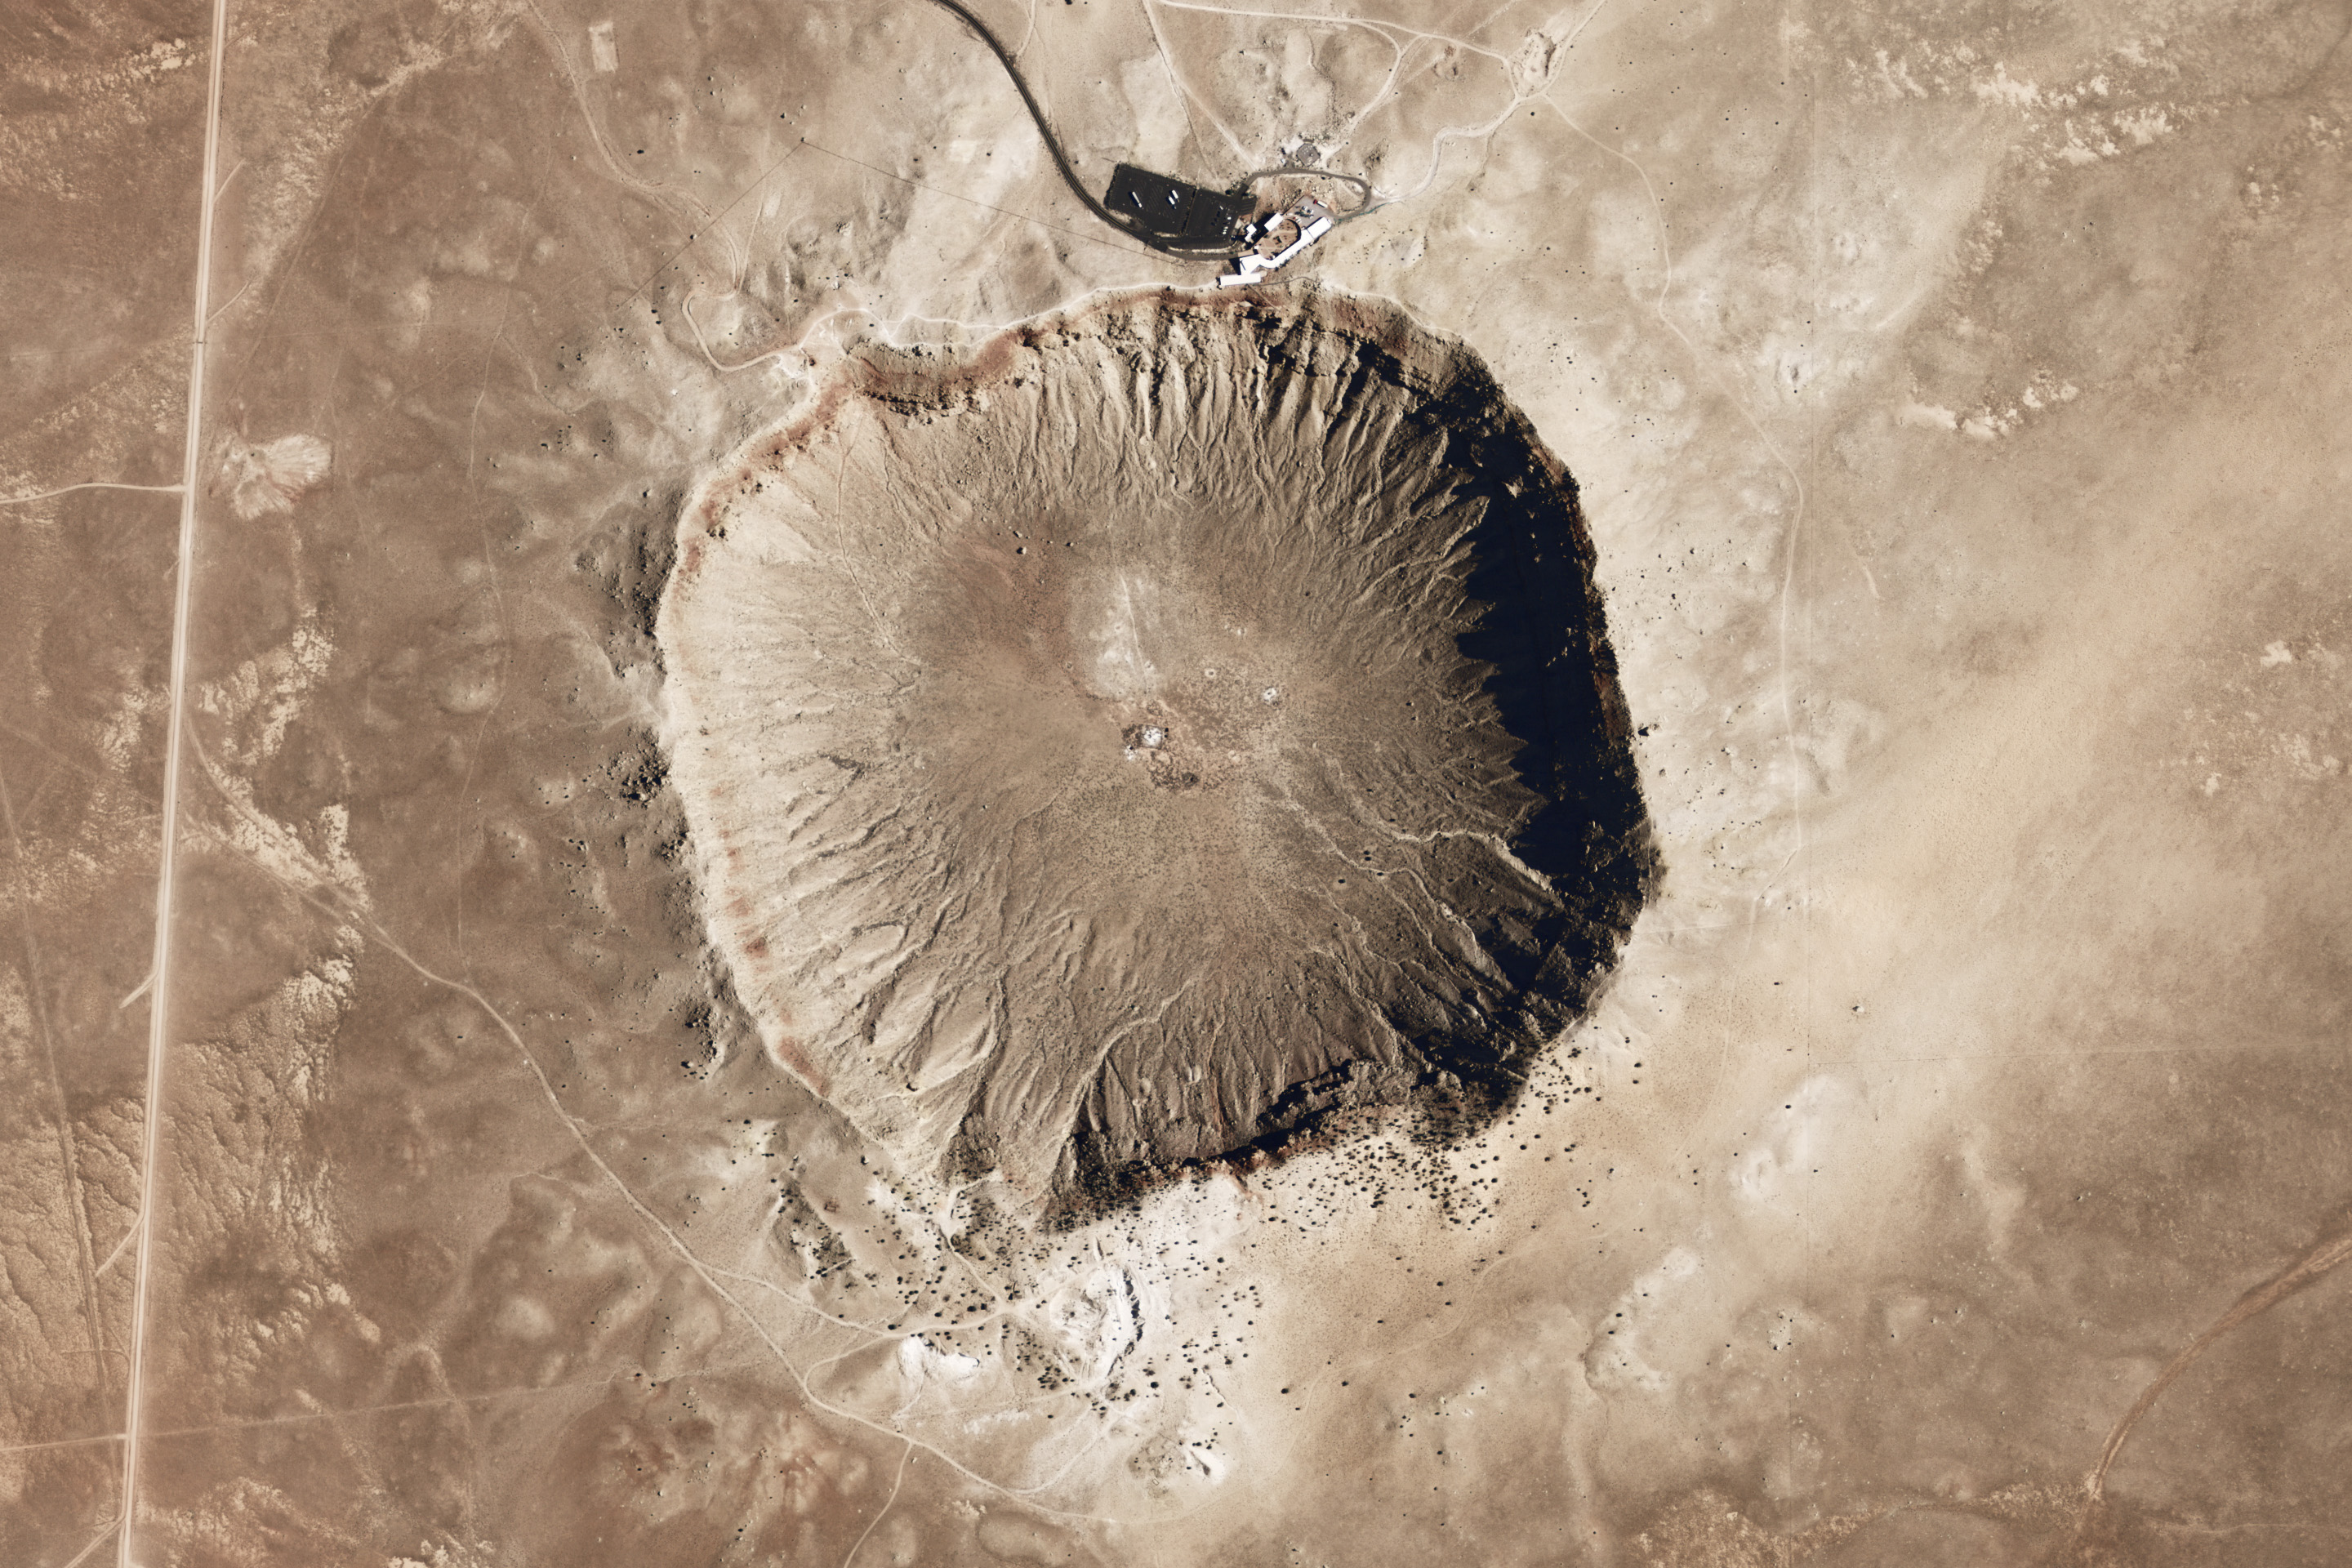
\includegraphics[width=\linewidth]{images/meteorcrater.jpg}
\subcaption{\textit{Meteor Crater, Arizona}. The classic example of a simple crater on Earth. Image from NASA's aircraft camera instrument. Image credit: NASA Earth Observatory. \ead[url]{http://earthobservatory.nasa.gov/IOTD/}. Accessed on December 2, 2013. \label{fig:meteorcrater}}\vspace{0.3cm}
\end{minipage}\\
\begin{minipage}{\linewidth}
\centering
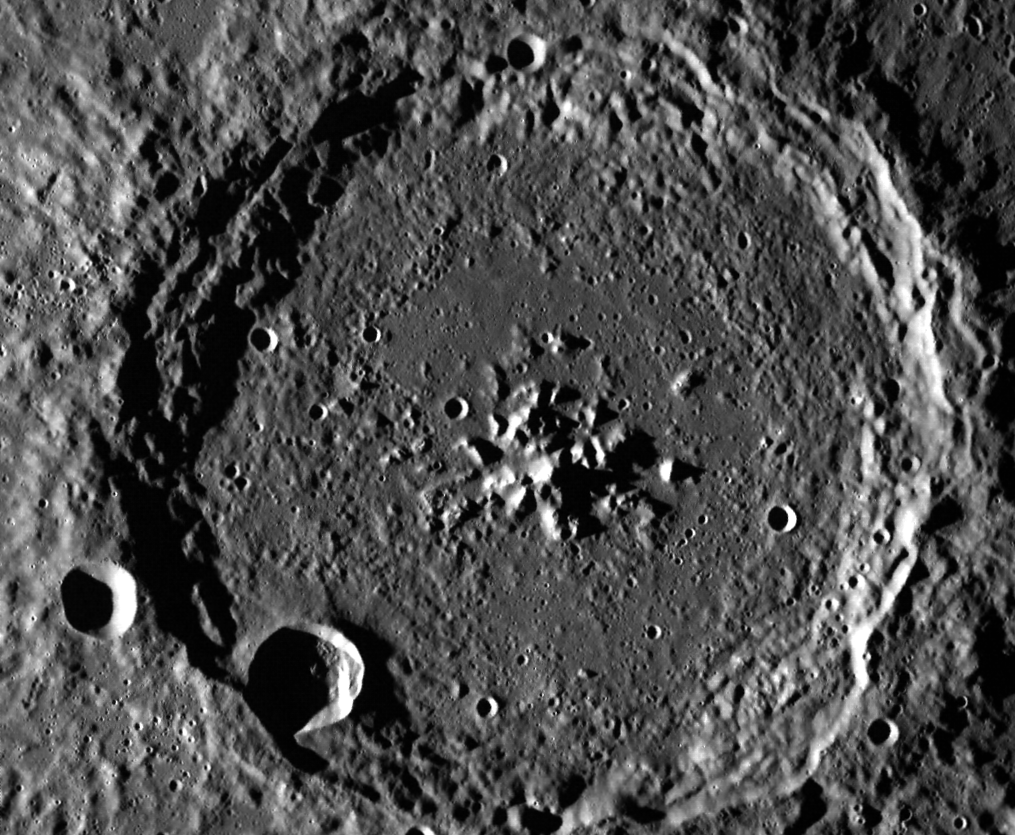
\includegraphics[width=\linewidth]{images/mercurycomplexcrater.png}
\subcaption{\textit{Verdi Crater, Mercury}. A complex crater on the surface of Mercury. Notice the central peak and collapsed, terraced rim. Image from NASA's Messenger's MDIS instrument. Image credit: NASA. \ead[url]{http://photojournal.jpl.nasa.gov/}. Accessed on December 2, 2013. \label{fig:mercurycrater}}
\end{minipage}
\caption{An example of a simple (\protect\subref{fig:meteorcrater}) and complex (\protect\subref{fig:mercurycrater}) central peak crater. \label{fig:simplecomplex}}
\end{figure}
%\pagebreak
%\newgeometry{left=4cm,bottom=2.5cm,top=2.5cm,right=2.5cm}

At the end of excavation, the transient cavity becomes known as the \textit{transient crater} \citep{osinski2012impact}. The form of the transient crater is defined using the maximum depth of the transient cavity during excavation, and the diameter at which surface material begins flowing inwards \citep{turtle2005impact}.\bigskip

It is the modification stage that has the biggest effect on the morphology of the final crater. Depending on the size of the projectile as well as the cohesion and gravity of the target, either a simple (Figure \ref{fig:meteorcrater}) or complex (Figure \ref{fig:mercurycrater}) crater will form. A complex crater is always larger than a simple crater, but has a significantly smaller depth to diameter ratio. While a simple crater tends to be bowl shaped, a complex crater often has a flat crater floor with a central peak/peak ring. The rim of a complex crater contains large terraced blocks of slumped material \citep{osinski2012impact}.\bigskip

Gravity is the main driving force behind the modification stage, with crater collapse occurring due to the unstable nature of the transient cavity \citep{melosh1999impact}. For a complex crater to collapse, the rock must be sufficiently weakened. To satisfy this, numerical models require that the rock be weakened to a much greater extent than standard rock mechanics predicts \citep{mckinnon1978investigation}. As a result, there are several models of structural weakening that attempt to explain complex crater rim collapse \citep{osinski2012impact}. Melosh developed the theory of \textit{acoustic fluidisation} in 1979 to explain this extraordinary weakening that occurs in a variety of natural phenomena, including complex crater collapse.

\subsection{Methods of Weakening \label{subsec:weakening}}


\begin{sloppypar}
There are several theories that attempt to explain the large drop in rock strength during a large impact event. Although a convenient summary of all theories are provided by \citet{osinski2012impact}, this thesis concerns itself with only two; the \textit{full model of acoustic fluidisation} \citep{melosh1979acoustic,melosh1996dynamical} and the \textit{block oscillation model} \citep{ivanov1997block}.
\end{sloppypar}

\subsubsection{The Full Model of Acoustic Fluidisation \label{sec:acfl}}

The full model of acoustic fluidisation, derived by \citet{melosh1979acoustic}, is a mechanical model which describes how temporal and spatial variations in acoustic vibrations induce rock weakening.\bigskip

Acoustic vibrations are generated by the shock wave during an impact event, and are scattered around the impact zone. These vibrations cause pressure fluctuations about the ambient overburden pressure. When the overall pressure drops below the ambient pressure, the materials yield strength is reduced, resulting in temporary weakening. Thus, over time, the rock material behaves as a viscous fluid. Equations \ref{eq:strain_rate} to \ref{eq:dedt} make up the full model of acoustic fluidisation. They describe the temporal and spatial varying properties of acoustic vibrations, and how these vibrations affect the strength of a material.\bigskip

Central to the theory of acoustic fluidisation is how the strain rate, $\dot{\epsilon}$, of a volume of acoustically fluidised material is related to the driving stress, $\tau$:

\begin{equation}\label{eq:strain_rate}
\dot{\epsilon} \approx \frac{\tau \psi}{\rho \lambda c_{p}} \left[ \frac{1-\erf\left(\chi\right)}{1+\erf\left(\chi\right)}\right],\vspace{0.2cm}
\end{equation}

where $\rho$ is the material density, $\lambda$ is the wavelength of the acoustic vibrations, and $\psi = (c_{p}/c_{s})^{2}$. $c_{p}$ and $c_{s}$ are the compressional wave velocity and shear wave velocity respectively. The error function argument, $\chi$, is given as:

\begin{equation} \label{eq:sc}
\chi = \frac{s_{c}}{\sigma}, \quad s_{c}=p-\frac{\tau}{\mu},\vspace{0.2cm}
\end{equation}

where $s_{c}$ is the critical pressure amplitude for sliding to occur, $p$ is the overburden pressure and $\mu$ is the coefficient of friction. $\sigma$ is the variance of the vibrational pressure, and is related to the acoustic energy density, $E$, via:

\begin{equation}
\sigma = c_{p} \rho \sqrt{2 E}.\vspace{0.2cm}
\end{equation}

Equation \ref{eq:strain_rate} can be modified by introducing the flow law for a Newtonian fluid, $\tau = 2 \eta \dot{\epsilon}$. This yields an equation describing an effective Newtonian viscosity \citep{collins2003acoustic}:

\begin{equation} \label{eq:eff_vis}
\eta_{\text{eff}} \approx \frac{\rho \lambda c_{p}}{2 \psi} \left[ \frac{1+\erf\left(\chi\right)}{1-\erf\left(\chi\right)} \right].\vspace{0.2cm}
\end{equation}

The full equation that describes the temporally and spatially varying acoustic energy is in the form of a non-linear, ordinary differential equation \citep{melosh1996dynamical}:

\begin{equation} \label{eq:dedt}
\frac{d E}{d t} = \frac{\xi}{4} \nabla^{2}E - \frac{c_{p}}{\lambda Q}E + e \tau_{ij} \dot{\epsilon}_{ij},\vspace{0.2cm}
\end{equation} 

where $\xi$ is the scattering diffusivity and $e$ is known as the regeneration parameter. $Q$ is the dissipation quality factor, formally defined as the  ratio of energy stored per cycle to the energy dissipated in that period \citep{collins2003acoustic,melosh1996dynamical}.\bigskip

The first term on the right hand side of equation \ref{eq:dedt} describes the diffusion of acoustic energy through the material. The second term describes the conversion of acoustic (elastic) energy into heat, hence it is a positive value subtracted from the rate of change of acoustic energy density. The final term in the differential equation acts to generate acoustic energy in regions with large stresses and strain rates. The regeneration parameter, $e$, holds a value between 0 and 1, and hence influences the efficiency of acoustic energy regeneration \citep{melosh1996dynamical}. Without the regeneration term, equation \ref{eq:dedt} would be linear, and thus the solution would be relatively easy to compute. However, the regeneration term causes the equation to be very non-linear, with an interesting, non-trivial solution.\bigskip

\subsubsection{The Block Oscillation Model}

The block model is an approximation to the \citet{melosh1979acoustic} model of acoustic fluidisation. It is derived from a simplified situation of acoustic fluidisation, where a single block slides over a surface \citep{ivanov1997block}. It assumes the region of the target is fractured into a series of large blocks, each separated by a matrix of smaller blocks. Acoustic vibrations, remnant from the shock wave, cause the larger blocks to oscillate, decreasing the stress and coefficient of friction between the blocks and the matrix \citep{collins2002numerical,ivanov1997block}. Consequently, sliding is induced between the blocks.\bigskip

\citet{melosh1999impact} showed that the rheological effects of the block model are similar to the Melosh model of acoustic fluidisation. However, the block model fails to induce distinct, fault sized zones of localised weakening into hydrocode simulations \citep{osinski2012impact}. The result is that the classic, discrete terracing associated with complex crater collapse has not been recreated in numerical simulations; instead, a smooth slumping occurs.

\subsection{The iSALE Hydrocode}

The impact model used to simulate crater formation in this research is known as iSALE, developed by Kai Wuennemann, Gareth Collins, and Dirk Elbeshausen. iSALE is essentially a model for simulating flow at all speeds, otherwise known as a hydrocode \citep{collins2002numerical}. Essentially, a hydrocode calculates the sum of all forces acting at a node, and applies the corresponding acceleration to either the node or material within a cell (depending on an Eulerian or Lagrangian frame of reference), in correspondence with Newton's second law. This process is carried out iteratively over all nodes in the model domain at incremental time steps. When the sum of all time steps reaches the final simulation time, the calculations stop \citep{collins2002numerical}.\bigskip

iSALE is a modified version of standard hydrocode because it also takes into account the rheological properties of the medium. This is very important for impact cratering; the final, modified crater produced hugely depends on the rheology of the target, which may change depending on the size, velocity, and strength of the projectile, among other factors.